\documentclass[a4paper]{article}
\usepackage[francais]{babel}
\usepackage{fontspec}
\usepackage{enumitem}
\usepackage{authblk}
\usepackage{minted}
\usepackage{amsmath}
\usepackage{hyperref}
\usepackage{tabularx}
\newcolumntype{C}[1]{>{\centering\arraybackslash}p{#1}}
\setlength{\parindent}{0pt}
\usepackage{hyperref}
\hypersetup{
    colorlinks,
    citecolor=black,
    filecolor=black,
    linkcolor=black,
    urlcolor=blue
}
\usepackage{etoolbox}
\patchcmd{\thebibliography}{\section*{\refname}}{}{}{}
\usepackage[left=2.5cm,top=2.5cm,right=2.5cm,bottom=2.5cm]{geometry}
\usepackage{glossaries}
	\let\oldnewacronym\newacronym
	\newcommand*{\provideacronym}[3]{%
	  \ifglsentryexists{#1}{%
	  }{%
	    \oldnewacronym{#1}{#2}{#3}%
	  }%
	}
\makeglossaries

\title{RustOS \protect\\ Système d’exploitation en Rust}
\author{Orphée Antoniadis}
\affil{\small Projet de Bachelor - Prof. Florent Glück}
\affil{\small Hepia ITI 3\up{ème} année}
\date{Semestre de Printemps 2017-2018}

\begin{document}
\maketitle

\begin{figure}[!b]
	\centering
	\begin{minipage}{.5\textwidth}
		\centering
		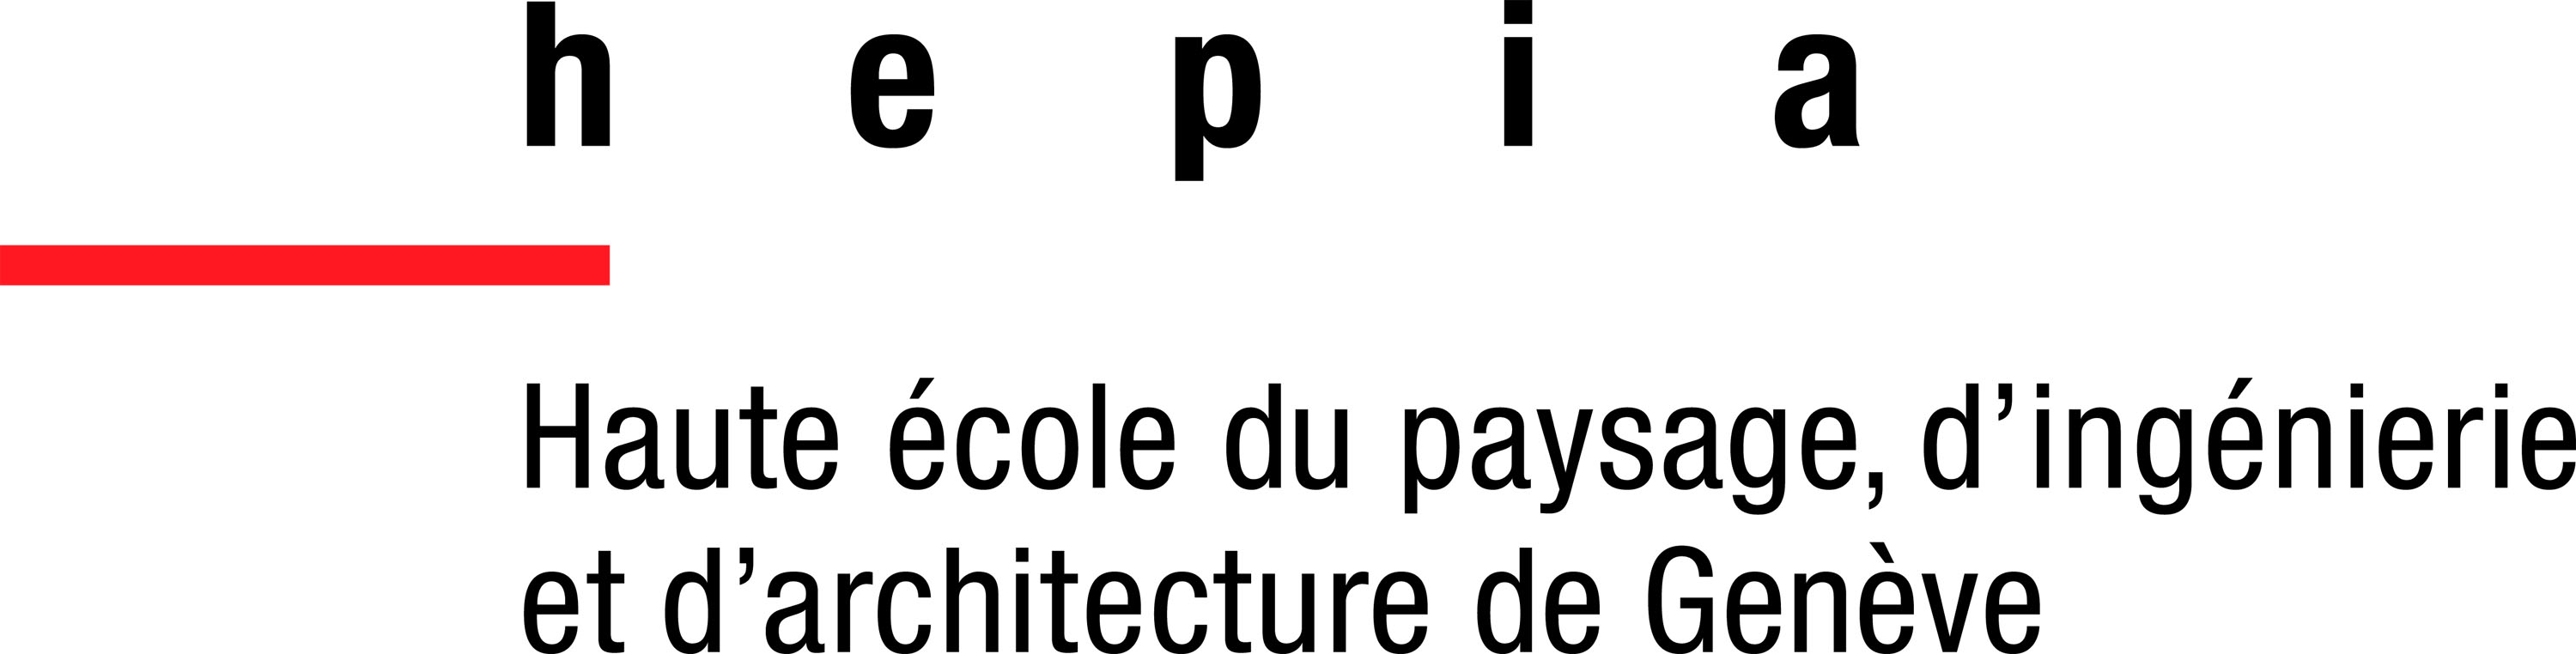
\includegraphics[width=.6\linewidth]{images/hepia.jpg}
	\end{minipage}%
	\begin{minipage}{.5\textwidth}
		\centering
		
\includegraphics[width=.6\linewidth]{images/hesso.jpg}
	\end{minipage}
\end{figure}
\newpage

\section*{Résumé}
Le but de ce projet est d’étudier le langage Rust, en particulier son utilisation
pour l’implémentation d’un système d’exploitation de type \textit{bare metal}. Le
langage Rust se révèle particulièrement intéressant en tant que digne successeur de C :
beaucoup plus robuste que ce dernier et potentiellement tout aussi rapide. La première
partie du projet sera de comprendre les paradigmes de programmation utilisés par
Rust ainsi que ses caractéristiques principales. Dans un deuxième temps, il s’agira
d’implémenter un système d’exploitation très simple, similaire à celui réalisé au
cours logiciel « Programmation système avancée » mais écrit en Rust plutôt qu’en C.

\newpage
\setcounter{tocdepth}{3}
\tableofcontents
\newpage
\listoffigures
\newpage

\section*{Remerciements}
\newpage

\section*{Convention typographique}
Lors de la rédaction de ce document, les conventions typographique ci-dessous ont
été adoptées.
\begin{itemize}[label=\textbullet]
	\item Tous les mots empruntés à la langue anglaise ont été écrits en \textit{italique}
	\item Toute référence à un nom de fichier (ou dossier), un chemin d’accès, une 
    utilisation de paramètre, variable, ou commande utilisable par l’utilisateur, 
    est écrite avec la police d’écriture \mintinline{rust}{Courier New}.
	\item Tout extrait de fichier ou de code est écrit selon le format suivant:
    \begin{minted}[linenos,frame=single,tabsize=4]{rust}
    fn main() {
        println!("Hello, world!");
    }
    \end{minted}
\end{itemize}
\newpage

\newacronym{os}{OS}{\textit{Operating System}}
\newacronym{elf}{ELF}{\textit{Executable and Linkable Format}}
\newacronym{gcc}{GCC}{\textit{GNU Compiler Collection}}
\newacronym{iso}{ISO}{\textit{International Organization for Standardization}}
\printglossary[type=\acronymtype,title={Acronymes}]
\newpage

%%%%%%%%%%%%%%%%%%%%%%%%%%%%%%%%%%%%%%%%%%%%%%%%%%%%%%%%%%%%%%%%%%
%%%%%%%%%%%%%%%%%%%%%%%%%%%%%%%%%%%%%%%%%%%%%%%%%%%%%%%%%%%%%%%%%%

\section{Introduction}
\subsection{Contexte}
% Rust
% Cours programmation avancée des systèmes

%%%%%%%%%%%%%%%%%%%%%%%%%%%%%%%%%%%%%%%%%%%%%%%%%%%%%%%%%%%%%%%%%%

\subsection{Objectif}

%%%%%%%%%%%%%%%%%%%%%%%%%%%%%%%%%%%%%%%%%%%%%%%%%%%%%%%%%%%%%%%%%%
%%%%%%%%%%%%%%%%%%%%%%%%%%%%%%%%%%%%%%%%%%%%%%%%%%%%%%%%%%%%%%%%%%

\section{Analyse}

%%%%%%%%%%%%%%%%%%%%%%%%%%%%%%%%%%%%%%%%%%%%%%%%%%%%%%%%%%%%%%%%%%
%%%%%%%%%%%%%%%%%%%%%%%%%%%%%%%%%%%%%%%%%%%%%%%%%%%%%%%%%%%%%%%%%%

\section{Conception}
\subsection{Environnement de développement}
La machine utilisée pour le développement du projet est un MacBook Pro avec un
processeur Intel à 3 GHz. Il a quand même fallut utiliser une machine virtuelle
(VMware) utilisant Linux (Ubuntu 16.04.4 LTS) pour la compilation. Ce choix a été
fait car il existe beaucoup plus de documentation sur l'implémentation de systèmes
d'exploitation sur Linux que sur Mac. Bien que Mac \acrshort{os} soit un système UNIX, les
exécutables générés sur cet environnement n'ont pas le même format que ceux générés
sur Linux qui sont au format \acrshort{elf}. Ceci rend le développement d'\acrshort{os} légèrement
différent sur Mac \acrshort{os}.

%%%%%%%%%%%%%%%%%%%%%%%%%%%%%%%%%%%%%%%%%%%%%%%%%%%%%%%%%%%%%%%%%%

\subsection{Technologies}
\subsubsection{Nasm}
Bien que le système d'exploitation développé devait être sur Rust, certaines parties
ont du être faites en assembleur car étant trop bas niveau pour le Rust. Ces éléments
seront décrits plus loin dans ce document. Nasm a été  utilisé pour compiler le
code assembleur x86 en \acrshort{elf} 32-bit. Nasm produit des fichiers objets pouvant être
liés à d'autres fichiers objets afin de créer un exécutable. \\

\subsubsection{Rustup}
Rust sera décrit plus en détails dans un prochain chapitre. Ce qu'il faut savoir
est que Rust est distribué sous trois versions différentes. La version \textit{stable},
la version \textit{beta} et la version \textit{nightly}. La version \textit{nightly}
possède plus de fonctionnalités mais sa stabilité n'est pas garantie. Cette version
a été utilisée pendant le développement du projet et l'utilitaire Rustup a été utilisé
pour son installation. Cet utilitaire permet de simplifier l'installation de Rust
quand on souhaite une version différente de la dernière version stable de Rust. \\

\subsubsection{Cargo et Xargo}
Lors du développement d'un système d'exploitation type \textit{bare metal}, on souhaite
s'affranchir de toute dépendance à une librairie externe. Tout doit être refait depuis
le début. Le code est donc compilé sans la bibliothèque standard (std). Rust a tout
de même besoin d'une base pour être compilé. Cette base est fournie par la librairie
\mintinline{rust}{core}. Cette librairie est minimale et permet de ne définir que
les primitives de Rust. Pour gérer les dépendences d'un projet Rust, il est conseillé
d'utiliser le gestionnaire de paquets cargo. Le problème est que cargo ne permet
pas de lier la librairie \mintinline{rust}{core} à un projet. Heureusement, un 
autre utilitaire basé sur cargo existe et permet d'installer par défaut la librairie
\mintinline{rust}{core} pour des projets sans bibliothèque standard. Cet utilitaire
se nomme xargo et est utilisé pour compiler le code Rust en fichiers objets \\

\subsubsection{Exécution du \textit{kernel}}
Le compilateur \acrshort{gcc} a été utilisé pour \textit{linker} les fichiers
objet générés par nasm et xargo. \acrshort{gcc} génère un fichier au format \acrshort{elf}. Pour utiliser
ce fichier comme un système d'exploitation \textit{bootable}, il faut en faire 
une image \acrshort{iso} \textit{bootable}. Pour se faire, l'utilitaire \mintinline{rust}{genisoimage}
est utilisé, couplé au \textit{bootloader} GRUB. L'image \acrshort{iso} est finalement exécutée
par la machine virtuelle QEMU. QEMU est une machine virtuelle pouvant émuler une
architecture. Pour ce projet, l'architecture i386 a été choisie afin d'émuler
un processeur Intel 32-bit.

%%%%%%%%%%%%%%%%%%%%%%%%%%%%%%%%%%%%%%%%%%%%%%%%%%%%%%%%%%%%%%%%%%

\subsection{Architecture}

%%%%%%%%%%%%%%%%%%%%%%%%%%%%%%%%%%%%%%%%%%%%%%%%%%%%%%%%%%%%%%%%%%
%%%%%%%%%%%%%%%%%%%%%%%%%%%%%%%%%%%%%%%%%%%%%%%%%%%%%%%%%%%%%%%%%%

\section{Rust}

%%%%%%%%%%%%%%%%%%%%%%%%%%%%%%%%%%%%%%%%%%%%%%%%%%%%%%%%%%%%%%%%%%
%%%%%%%%%%%%%%%%%%%%%%%%%%%%%%%%%%%%%%%%%%%%%%%%%%%%%%%%%%%%%%%%%%

\section{Système d’exploitation de type \textit{bare metal}}
\subsection{Compilation}
Quand on veut compiler un simple code C en utilisant \acrshort{gcc} par
exemple, le compilateur passe par plusieurs étapes. Le préprocesseur génère d'abord
un fichier C en fonction des directives de préprocesseur. Ce fichier C est ensuite
compilé en code assembleur qui est lui même compilé en code objet. Le \textit{linker}
permet ensuite de lier les différents fichiers objets et générer un exécutable.
Nous avons déjà eu un aperçu des différentes étapes de la compilation d'un \acrshort{os}
de type \textit{bare metal} dans la partie 3.2. A la différence de la compilation
d'un code C, nous avons d'un côté du code assembleur et de l'autre du code Rust.
Nasm et cargo permettent tous deux de générer des fichiers objets. Il n'y a donc
que la dernière étape à effectuer ce que \acrshort{gcc} permet de faire avec
la commande suivante.
\begin{minted}[tabsize=4]{bash}
gcc $(OBJS) -T $(LINKER) -static -m32 -ffreestanding -nostdlib -o $@ $(RUST)
\end{minted}
Ici, \mintinline{shell}{$(OBJS)} représente les fichiers objets générés par
\mintinline{rust}{nasm}, \mintinline{shell}{$(LINKER)} est un fichier permettant
de faire l'édition des liens et \mintinline{shell}{$(RUST)} représentre les fichiers
objets générés par Rust.

%%%%%%%%%%%%%%%%%%%%%%%%%%%%%%%%%%%%%%%%%%%%%%%%%%%%%%%%%%%%%%%%%%

\subsection{\textit{Linking}}

%%%%%%%%%%%%%%%%%%%%%%%%%%%%%%%%%%%%%%%%%%%%%%%%%%%%%%%%%%%%%%%%%%

\subsection{Processus de \textit{boot}}

%%%%%%%%%%%%%%%%%%%%%%%%%%%%%%%%%%%%%%%%%%%%%%%%%%%%%%%%%%%%%%%%%%

\subsection{Adressage mémoire}

%%%%%%%%%%%%%%%%%%%%%%%%%%%%%%%%%%%%%%%%%%%%%%%%%%%%%%%%%%%%%%%%%%

\subsection{Ports}

%%%%%%%%%%%%%%%%%%%%%%%%%%%%%%%%%%%%%%%%%%%%%%%%%%%%%%%%%%%%%%%%%%

\subsection{Interruptions}

%%%%%%%%%%%%%%%%%%%%%%%%%%%%%%%%%%%%%%%%%%%%%%%%%%%%%%%%%%%%%%%%%%

\subsection{Periphériques}
\subsubsection{VGA}

\subsubsection{\textit{Timer}}

\subsubsection{Clavier}

%%%%%%%%%%%%%%%%%%%%%%%%%%%%%%%%%%%%%%%%%%%%%%%%%%%%%%%%%%%%%%%%%%
%%%%%%%%%%%%%%%%%%%%%%%%%%%%%%%%%%%%%%%%%%%%%%%%%%%%%%%%%%%%%%%%%%

\section{Système de fichiers}
\subsection{Introduction}

%%%%%%%%%%%%%%%%%%%%%%%%%%%%%%%%%%%%%%%%%%%%%%%%%%%%%%%%%%%%%%%%%%

\subsection{Structure}

%%%%%%%%%%%%%%%%%%%%%%%%%%%%%%%%%%%%%%%%%%%%%%%%%%%%%%%%%%%%%%%%%%
%%%%%%%%%%%%%%%%%%%%%%%%%%%%%%%%%%%%%%%%%%%%%%%%%%%%%%%%%%%%%%%%%%

\section{Résultats}

%%%%%%%%%%%%%%%%%%%%%%%%%%%%%%%%%%%%%%%%%%%%%%%%%%%%%%%%%%%%%%%%%%
%%%%%%%%%%%%%%%%%%%%%%%%%%%%%%%%%%%%%%%%%%%%%%%%%%%%%%%%%%%%%%%%%%

\section{Discussions}
\subsection{Problèmes rencontrés}

%%%%%%%%%%%%%%%%%%%%%%%%%%%%%%%%%%%%%%%%%%%%%%%%%%%%%%%%%%%%%%%%%%

\subsection{Améliorations possibles}

%%%%%%%%%%%%%%%%%%%%%%%%%%%%%%%%%%%%%%%%%%%%%%%%%%%%%%%%%%%%%%%%%%
%%%%%%%%%%%%%%%%%%%%%%%%%%%%%%%%%%%%%%%%%%%%%%%%%%%%%%%%%%%%%%%%%%

\section{Conclusion}

\newpage

%%%%%%%%%%%%%%%%%%%%%%%%%%%%%%%%%%%%%%%%%%%%%%%%%%%%%%%%%%%%%%%%%%
%%%%%%%%%%%%%%%%%%%%%%%%%%%%%%%%%%%%%%%%%%%%%%%%%%%%%%%%%%%%%%%%%%

\section{Références}
\nocite{*}
\bibliographystyle{unsrt}
\bibliography{biblio}

\end{document}
